\documentclass[final]{beamer}
\begin{filecontents}{postertemplate.bib}

\end{filecontents}
\usetheme{PSI}
\usepackage{natbib}
\usepackage{ragged2e}   % package for justifying
%\usepackage[demo]{graphicx}
\usepackage{subcaption}
\addtobeamertemplate{block begin}{}{\justifying}  %new code
\bibliographystyle{abbrv}
\usepackage[orientation=portrait,size=a0,scale=1.4,debug]{beamerposter}
\usepackage[absolute,overlay]{textpos}
\setlength{\TPHorizModule}{1cm}
\setlength{\TPVertModule}{1cm}

\title{Voice Control for a Gripper Using Mel-Frequency Cepstral Coefficients and Gaussian Mixture Models}
\author{Velasco-Hernandez, Gustavo $^{1}$. D\'{i}az-Toro, Andr\'{e}s Alejandro $^{2}$}
\institute{Perception and Intelligent Systems Research Group\\
	School of Electric and Electronics Engineering\\
	Universidad del Valle}
\footer{Contact:\\ 1. velasco.gustavo@correounivalle.edu.co\\ 2. andres.a.diaz@correounivalle.edu.co}
\date{}

\hyphenation{performance}
\begin{document}
\begin{frame}{}

\begin{textblock}{5}(3,3)

\includegraphics[width=0.10\paperwidth]{figs/univalle.png}
\end{textblock}
\begin{textblock}{5}(70,5.5)

\includegraphics[width=0.15\paperwidth]{figs/psilogo3.png}
\end{textblock}


\begin{textblock}{39.5}(1,19)
\begin{block}{Abstract}
This work presents an implementation of a speaker-dependent speech recognition system used to control a gripper. The application was made using MATLAB and the gripper was assembled using the Lego Mindstorm NXT robotic kit. Four commands are implemented for controlling the gripper: Open, close, rotate left and rotate right. The development was divided into two stages. In training stage, we use Mel Frequency Cepstral Coefficients (MFCCs) and Gaussian Mixture Models (GMMs) to generate a representation of each defined command. Then, in testing stage, those models are used to identify the speaker’s utterance and send the command to the actuator. Finally, we present test results that show a performance of 95.09\% for our system, and then we compare it with similar works.
\end{block}

\begin{block}{Methodology}

The methodology developed along this work is based on two main features. The first one is that the system is focused on detecting isolated words; this means that the speaker will say words separated by silence spaces. The second feature is that the system detects words only for the speaker for whom the models were computed.

\begin{columns}[t]
\column{.5\textwidth}
\centering
\begin{figure}
	%\begin{subfigure}{.24\paperwidth}
	%\begin{center}
	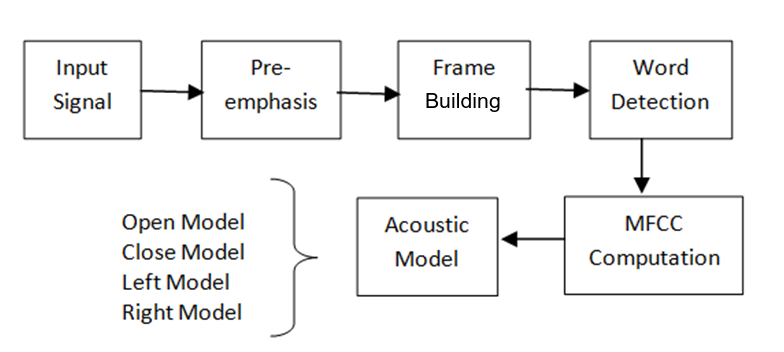
\includegraphics[width=0.8\linewidth]{figs/1bloquesTraining}
	%\end{center}
    \caption{Training Stage.}
	\label{trainingBlocks}
	\end{figure}
\column{.5\textwidth}
\centering
\begin{figure}	
	%\begin{subfigure}{.24\paperwidth}
	%\begin{center}
    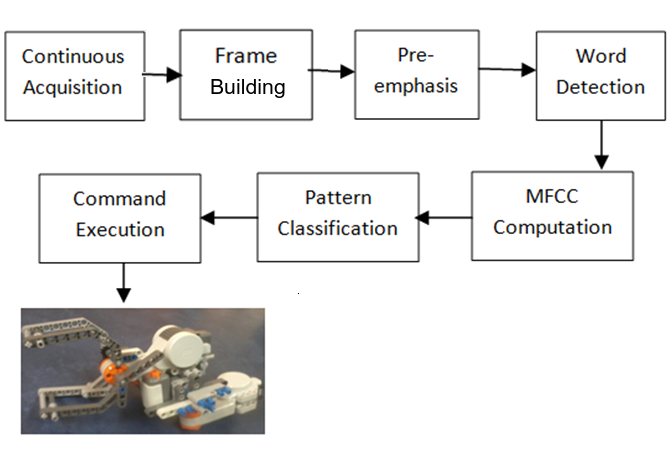
\includegraphics[width=0.8\linewidth]{figs/11bloquesTesting}
	%\end{center}
    \caption{Testing Stage.}
	\label{trainingBlocks}

\end{figure}
\end{columns}
\end{block}


\end{textblock}

\begin{textblock}{39.5}(43.05,19)

\begin{block}{Results}

\begin{table}[h]
\centering
%\tiny
%\scriptsize
\footnotesize
%\small
\begin{tabular}{||p{3.5cm}||p{4cm}||p{3cm}||p{4cm}||p{4cm}||p{4cm}||p{4cm}||p{6cm}||}%p{3cm}
\hline 
\textbf{Speaker} &  \textbf{GMM Number} & \textbf{No. of words} & \multicolumn{4}{|c||}{\textbf{Command Performance (\%)}} & \textbf{Global Performance (\%)}\\
\cline{4-7}
& & & \textbf{Open} & \textbf{Close} & \textbf{Left} & \textbf{Right} & \\
\hline \hline

1 &5 &17 &94.11 &100 &94.11 &100 & \textbf{97.05} \\
\hline 
1 &8 &17 &100 &88.23 &82.35 &94.11 &\textbf{88.23} \\
\hline
1 &11 &17 &94.11 &82.35 &82.35 &94.11 &\textbf{88.23} \\
\hline
2 &5 &18 &100 &94.11 &94.11 &100 & \textbf{97.05}\\
\hline
2 &8 &16 &100 &100 &100 &100 & \textbf{100}\\
\hline
2 &11 &18 &100 &100 &100 &100 & \textbf{100}\\
\hline

\end{tabular}
\caption{Performance of the Voice Recognition System}
\label{performance}
\end{table}

\begin{table}[!ht]
	\small
	\begin{center}	
	\begin{tabular}{|c | p{17.5cm} | c|}
	\hline
	\textbf{Approach} & \textbf{Description} & \textbf{Performance} \\
	\hline
	\hline
	Tezer \cite{Tezer} &
		Used LPC and DTW. Implemented in MATLAB. &
		86\% \\
	Beritelli \cite{Beritelli} &
		Used VQ. Proposed to noise-robust application &
		~92\% \\
	Bedoya \cite{Bedoya} &
		Used wavelts, HMMs and MFCCs &
		98\% \\
	Phokharatkul \cite{Phokharatkul} &
		Used filter banks and Mel scale analysis &
		96.3\% \\
	Ali \cite{Ali} &
		Used MFCCs and ANN. Isolated or continuous speech mode &
		~96\% \\
	Chin \cite{Chin} &
		Used MFCCs and ANN&
		98.9\% \\
	Ours &
		Used MFFCs and GMMs, implemented in MATLAB &
		95.09\%\\
	\hline
	\end{tabular}
	\end{center}	
	\caption{Comparision of different speech recognition systems}
	\label{table_comp}
\end{table}

\end{block}

\begin{block}{Conclusions}
In this paper we presented an speaker-dependent speech recognition system based on Mel Frequency Cepstral Coefficients (MFCCs) for extracting features and Gaussian Mixture Models (GMMs) for creating the model of each command. We test the systems with two different speakers and the worst case was $91.17\%$ (average of global performance for speaker $1$) of accuracy for a speaker. For a particular command, the worst case was $82.35\%$ and the average of the global performance of the system was $95.09\%$ (see Results section).

As future work, we propose the evaluation of the system with more than four commands and the creation of models with utterances from different speakers in order to test the capability of the system to be speaker-independent.
\end{block}

\begin{block}{References}
\small
\bibliography{postertemplate.bib}
\end{block}

\end{textblock}

\end{frame}
\end{document}
